\documentclass[landscape,a4paper,12pt,french, twocolumn]{article}

\usepackage{../../Style}

\renewcommand\tabularxcolumn[1]{m{#1}}

\begin{document}

\title{\vspace{-1cm} Les nombres réels \vspace{-1cm} }
\date{}
\maketitle

\begin{FlushLeft}

\thispagestyle{empty}

\section{Les ensembles de nombres}


\subsection{Les entiers}

$\N$ désigne l’ensemble des entiers positifs ou nuls, appelés entiers naturels. $0$ est un entier naturel, on note $0 \in \N$. Par contre, $-3$ n'en est pas un, on note $-3 \not\in \N$.
$$ \N = \left\{ 0;1;2; \ldots \right\}$$

$\Z$ désigne l’ensemble des entiers négatifs, positifs ou nuls, appelés entiers relatifs: $1 \in \Z, -2 \in \Z$ mais $0.5 \not\in \Z$.
$$ \Z = \left\{ \ldots ; -2 ; -1 ; 0 ; 1 ; 2 ; \ldots \right\}$$

Tout entier naturel est aussi un entier relatif. L'ensemble $\N$ est donc inclus dans l'ensemble $\Z$. On note $\N \subset \Z$.

\subsection{Les nombres décimaux}

Un nombre décimal est un nombre qui peut s’écrire avec un nombre fini de chiffres après la virgule. Autrement dit, un nombre décimal peut s’écrire sous la forme $\frac a {10^n}$, où $a \in \Z$ et $n \in \N$. On note $\D$ l’ensemble des nombres décimaux.
$$0.5=\frac 5 {10} \in \D,\ 1/4=0.25 \in \D,\ \frac 1 3=0.333 \ldots \not\in \D$$

Tout entier relatif est aussi un entier décimal: $\Z \subset \D$: Par exemple, $-1 = \frac {-1} 1 = \frac {-1} {10^0}$.

\subsection{Les nombres rationnels}

Un nombre rationnel est un nombre qui peut s’écrire sous la forme $\frac p q$, où $p$ et $q$ sont des entiers relatifs et $q$ est non nul. On note $\Q$ l’ensemble des nombres rationnels.
$$-2 = \frac {-2} 1 \in \Q,\ \frac 1 3 \in \Q,\ \frac 3 7 \in \Q,\ \sqrt 2 \not\in \Q$$

\
\begin{prop} \ 
\begin{itemize}
\item Tout nombre rationnel non nul admet une seule écriture fractionnaire irréductible
\item Si un nombre est rationnel, alors son développement décimal est périodique à partir d’un certain rang. La réciproque est aussi vraie.
\end{itemize}

\end{prop}

Par exemple, $x=0.0909 \ldots$ est rationnel: $100x=9.0909 \ldots$ donc $100x - x = 9$ d'où $99x=9$ puis $x= \frac 9 {99} = \frac 1 {11}$.

Tout nombre décimal est aussi un nombre rationnel: $\D \subset \Q$.

\subsection{Les nombres réels}

$\R$ désigne l’ensemble des nombres connus en classe de seconde, qu’on appelle nombres réels. De plus, un nombre réel qui n’est pas rationnel est dit irrationnel.
$$ \sqrt 2, \pi, \sqrt { \sqrt { \pi } } \text{ sont irrationnels}$$

On représente l’ensemble des nombres réels sur une droite graduée:

\begin{center}
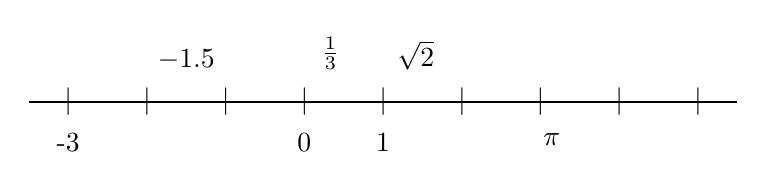
\begin{tikzpicture}[>=latex]
    \draw[thick,-] (-3.5,0) --(5.5,0);
    \node[below=8pt] at (0,0) {0};
    \node[below=8pt] at (1,0) {1};
    \node[below=8pt] at (-3,0) {-3};
    \node[above=8pt] at (1.414,0) {$\sqrt 2$};
    \node[] at (1.414,0) {$\shortmid$};
    \node[below=8pt] at (3.142,0) {$\pi$};
    \node[] at (3.142,0) {$\shortmid$};
    \node[above=8pt] at (0.33,0) {$\frac 1 3$};
    \node[] at (0.33,0) {$\shortmid$};
    \node[above=8pt] at (-1.5,0) {$-1.5$};
    \node[] at (-1.5,0) {$\shortmid$};
    \foreach \xp in {-3,-2,...,5}{\node[] at (\xp,0) {$\mid$};}
   
\end{tikzpicture}
\end{center}

Enfin, on remarque que tous ces ensembles sont inclus les uns dans les autres: $\N \subset \Z \subset \D \subset \Q \subset \R$.

\end{FlushLeft}

\end{document}
